\RequirePackage{luatex85}
\documentclass{standalone}
\usepackage{tikz}

% Color Definitions
\definecolor{SourceColor}{RGB}{85,168,104}
\definecolor{TargetColor}{RGB}{221,132,82}
\definecolor{TargetChangerColor}{RGB}{255,153,0}
\definecolor{AbsorbingAreaColor}{RGB}{196,78,82}
\definecolor{ObstacleColor}{RGB}{179,179,179}
\definecolor{StairColor}{RGB}{129,114,178}
\definecolor{MeasurementAreaColor}{RGB}{255,0,0}
\definecolor{InformationAreaColor}{RGB}{0,100,20}
\definecolor{AerosolCloudColor}{RGB}{202,156,76}
\definecolor{AgentColor}{RGB}{76,114,202}
\definecolor{AgentIdColor}{RGB}{255,127,0}

\newcommand{\MeasurementAreaOpacity}{0.549020}
\newcommand{\AerosolCloudOpacity}{0.039216}
\usetikzlibrary{shapes,arrows,chains}


\begin{document}

\begin{tikzpicture}
\node[] at (0,0) {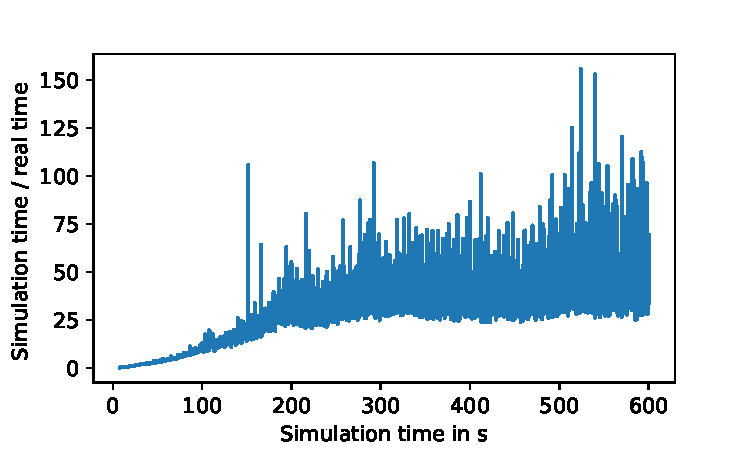
\includegraphics[width=7.8cm,height=6.5cm, trim={0.5cm 0.5cm 0 0}, clip]{./RatioSimulationTimeRealTime.pdf}};
\node[] at (7.2,0) {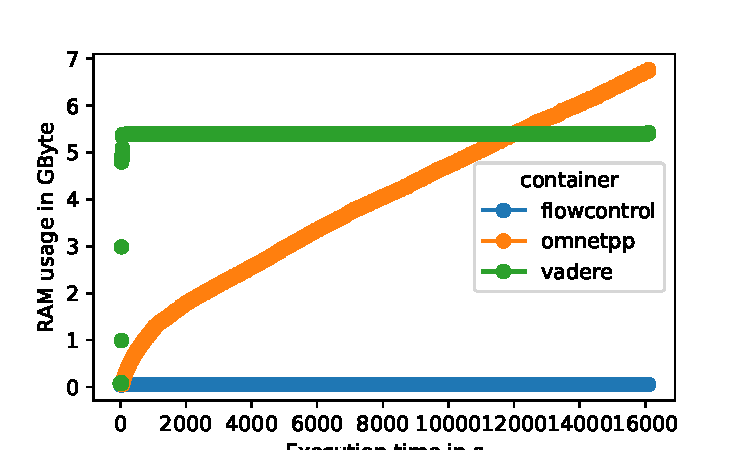
\includegraphics[width=7cm,height=6.3cm, trim={1.0cm 0.3cm 1.2cm 0cm}, clip]{./RAMUsageGByte.pdf}};
\node[] at (0,-3.5) {Simulation time in s};
\node[] at (7.5,-3.5) {Execution time in s};
\node[font=\small] at (11,-2.94) {$\cdot 10^3$};
\node[fill=white,font=\small] at (0,-3.0) {~0~\,~~~100~\,~~~200~~\,~~300~~\,~~400~~\,~~500~~\,~~600~};
\node[rotate=90] at (-4.1,-0.3) {Realtime / simulation time};
\node[rotate=90] at (3.5,-0.3) {RAM usage in GByte};
\node[fill=white,font=\small] at (7.4,-3.0) {~0 ~\,~~~2  ~\,~~ 4 ~~~ 6 ~~~ 8 ~~~ 10 ~~\,12 ~~  14 ~~ 16~~};
\node[fill=white,font=\small] at (9.3,0.5) {Container};
\end{tikzpicture}
\end{document}
